% Allow relative paths in included subfiles that are compiled separately
% See https://tex.stackexchange.com/questions/153312/
\providecommand{\main}{..}
\documentclass[\main/thesis.tex]{subfiles}
\onlyinsubfile{\zexternaldocument*{\main/tex/introduction}}

\begin{document}
\chapter{On-line Drum Programming}
\section{Suitability for Live Performance}
One use case for the drum generation approach pursued in this work is to create and evolve drum-tracks  on  the  fly. With our generative system of drums in place, we implemented a program which perpetually evolves a given drum-pattern (or rhythm) by continually replacing the drum sounds within the pattern by the outputs of the TPE system. This program is outlined in Figure~\ref{fig:live_dru}. This approach could be particularly interesting in a live setting where drum-patterns are repeated for long durations. In order to test this approach, we created a basic music notation where we consider a drum-pattern program to have the following attributes:

\begin{itemize}
    \item Beats Per Minute (BPM): This defines the "speed" of the pattern. 
    \item Number of Beats: How many beats are in the pattern.
    \item Drum Pattern: An action must be taken at each beat, either a drum is played or no action is taken and nothing is played for that beat. A drum pattern dictates what action is taken at each beat.
\end{itemize}

We defined a basic 8 beat drum pattern\footnote{The actions taken at each beat are kick-snare-hat-kick-snare-hat-shaker sequentially} at 160 BPM, and  implemented  a  program  which  perpetually  listens for new outputs from the TPE system and creates drum tracks according to the pre-determined drum pattern.  Whenever a new drum is created, a drum track is generated using a drum-kit of the latest outputs. To test this approach, we let the program run for 100,000 iterations of the TPE generative system (i.e., 100,000 random sounds are synthesized and tested for similarity to drum sounds using our best models). 980 of the 100,000 attempts resulted in the generation of a drum sound, therefore this process gave us 980 drum tracks. If listened to sequentially, one of the drum types in the drum-kit is modified before rendering each drum track, but all drum-tracks are identically programmed. These drum tracks are available for download on Zenodo\footnote{https://zenodo.org/record/5004327}.

\begin{figure}[htpb]
    \begin{center}
    \textbf{Drum Track Generation}
    \makebox[\textwidth]{
    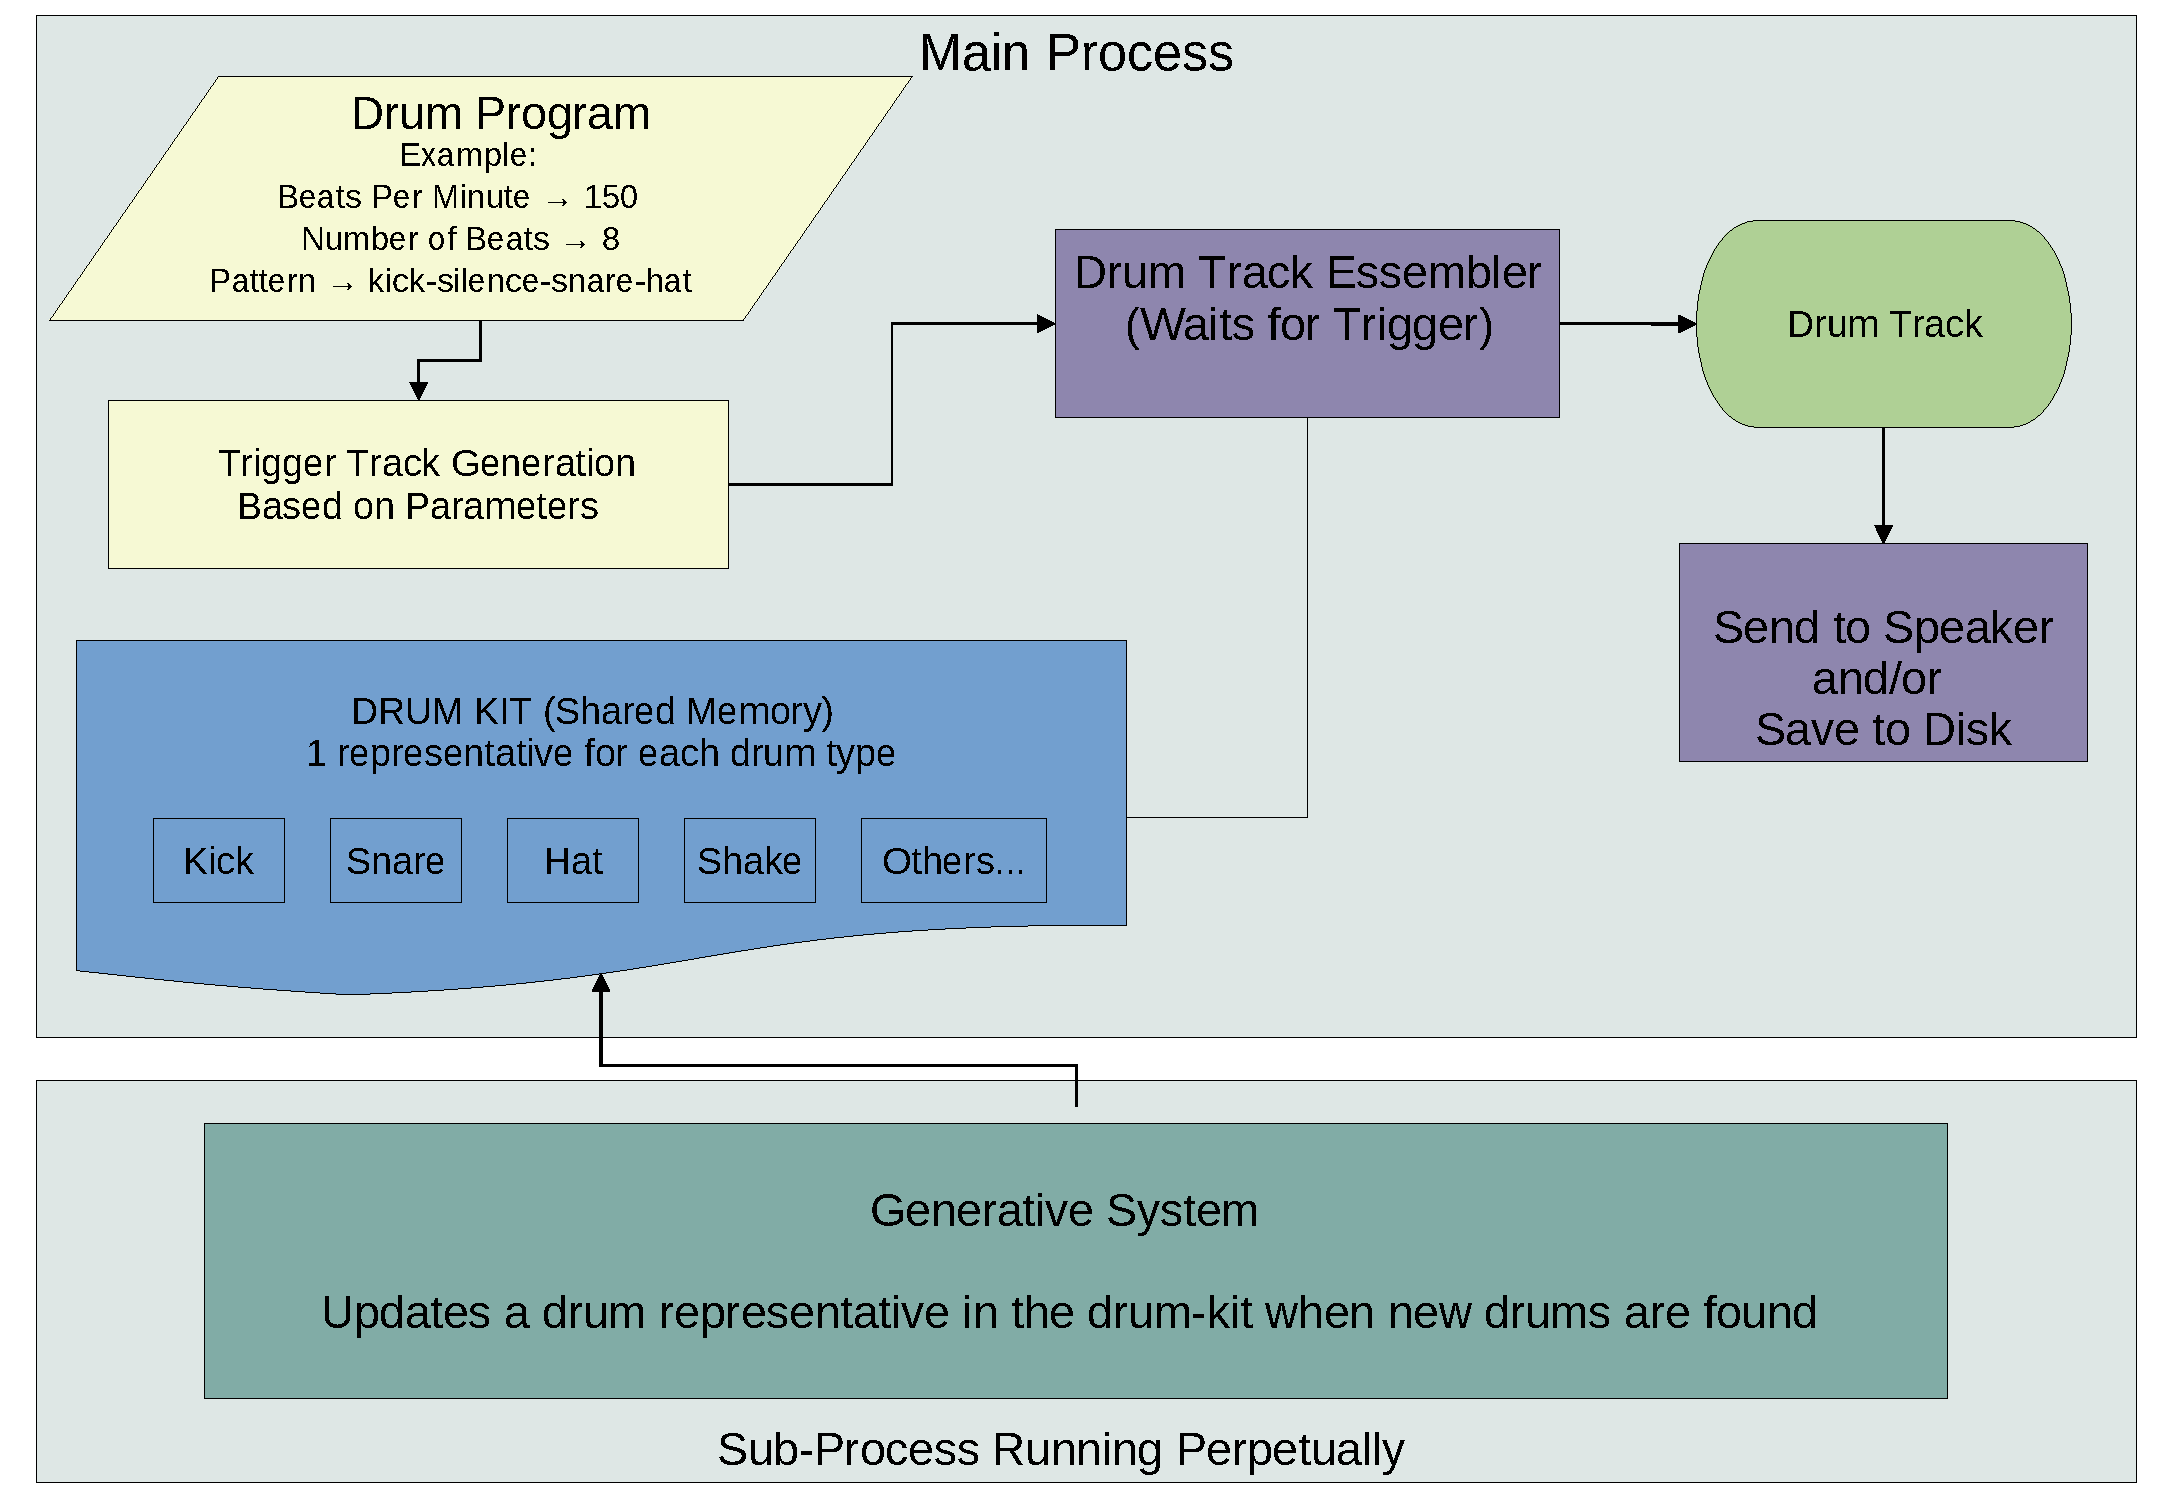
\includegraphics[width=1.1\linewidth]{images/live_programming.pdf}}
    \end{center}
    \caption{Live drum programming outline. Given a pre-defined drum program, the main process creates drum tracks using a drum-kit. This drum-kit is continually modified by a generative system running in a background process. In a live setting, the drum track assembler can be triggered at set times depending on the program, in offline generation, it can be triggered whenever there is a modification to the drum-kit.  }
\label{fig:live_drumming}
\end{figure} 

\section{Analyzing the Outputs}

\section{Conclusion}
Beyond improvements in the models themselves, these drum-tracks highlight other important avenues for enhancement of the system.  We believe that the expansion of the synthesizer parameters is needed to create larger variety of sounds. Another issue  with  usability  is  that  stricter,  more  powerful  drum  vs  non-drum  classifiers may reject nearly all synthesized outputs, making the creation of new drum-kits time consuming if not impossible.  In this case, 100,000 attempts were made at creating a drum,  985 of which were successful, leading to 985 different drum tracks. 

This means that the introduction of an algorithm which intelligently  modifies  parameters  in  order  to  bypass  the  drum  vs  non-drum classifier will be a necessary step in the future to create desired sounds more efficiently.
\end{document}